%%%%%%%%%%%%%%%%%%%% author.tex %%%%%%%%%%%%%%%%%%%%%%%%%%%%%%%%%%%
%
% sample root file for your "contribution" to a proceedings volume
%
% Use this file as a template for your own input.
%
%%%%%%%%%%%%%%%% Springer %%%%%%%%%%%%%%%%%%%%%%%%%%%%%%%%%%


\documentclass{svproc}
%
% RECOMMENDED %%%%%%%%%%%%%%%%%%%%%%%%%%%%%%%%%%%%%%%%%%%%%%%%%%%
%

% to typeset URLs, URIs, and DOIs
\usepackage{url}
\usepackage[english]{babel}
\selectlanguage{english}
\usepackage[utf8]{inputenc} 
\usepackage{graphicx}    % can use native umlauts

\def\UrlFont{\rmfamily}

\begin{document}
\mainmatter              % start of a contribution
%
\title{Predicting Contamined PCR Plates in a Metagenomic Sequencing Study}
%
\titlerunning{Effects of contamined PCR plates}  % abbreviated title (for running head)
%                                     also used for the TOC unless
%                                     \toctitle is used
%
\author{Maximilian Joas\inst{1} }
%
%\authorrunning{$<$Joas$>$ et al.} % abbreviated author list (for running head)
%
%%%% list of authors for the TOC (use if author list has to be modified)
\tocauthor{Maximilian Joas}
%
\institute{Universität Leipzig\\Machine Learning Group\\Leipzig, Germany\\
\email{mj13body@studserv.uni-leipzig.de}}
%
\maketitle              % typeset the title of the contribution
%
\begin{abstract}
    Geben Sie Ihrer Ausarbeitung einen möglichst aussagekräftigen Titel und fassen Sie Ihre Arbeit \textit{nach Fertigstellung des eigentlichen Berichts} noch einmal an dieser Stelle so kurz wie möglich zusammen. Versuchen Sie dabei folgende Aspekte jeweils mit einem Satz (maximal zwei Sätze) zusammenzufassen: Fragestellung, Methodik, Ergeb\-nisse, Schlussfolgerungen. Die Zusammenfassung muss nicht voll\-ständig sein, sondern sollte in erste Linie so klar wie möglich herausstellen, warum es sich lohnt, die vorliegende Arbeit vollständig zu lesen.
    \keywords{Maschinelles Lernen, Empirische Daten, Wissenschaftliches Arbeiten}
\end{abstract}
%
%
\section{Research Question}
%
Advances and cost reduction of sequencing expirements had an vast impact on the field of Metagenomics (research that focuses on many genomes at the same time). The vast amount of data obtained from whole genome sequencing experiments in metegenomic leads to oppurtunities in pathogen detection, ecological studies and drug development \cite{THREE OPNE TABS}. On the other had the abundance of data poses challenges to the analysis of metagenomic data. Consequently, classical statistical methods reach their limits and other approaches such as machine learning are often used \cite{Paperunde}.\\


Not only the amount of data, but also the type of data are challenging, on top of that the technical prorcess of sequencing can lead to problems.
In particular, contamination an noise are important problems when studying metagenomics \cite{paper Michel}. Noised up and or contmained data can lead to false conclusions in experiments. Therefore it would be valuable to predict contamination on PCR plates and find factors that are distinctive to contamined PCR plates. In this article I will investigate if it is possible to predict contamined PCR plates based on OTU counts as well as meta data. Furhtermore I will present factors that distinghuis contamined from not contamined PCR plates with the help of machine learning.


\section{State of the Art}
Machine learnig methods have benn successfully used in the study of metagenomics data  \cite{paperrunde}. However, specifically on my research question there are, to the best of my knowledge no publications. Nevertheless, this section aims to give an overview of the state of the art of the implemented methods. In general, machine learning methods are distinguished in supervised and unsupervised methods. In the case of supervised learning there is a known mapping metween input and target variable and the methods learn the assocation and can predict the output variable for new data. In this case the target variable is if the PCR plate is contamined.
TODO

 
%
%
\section{Methodik}
%
\subsection{Conception}
TODO CLEAR SEPARATION BETWEN META DATA AND DATA, BASELINE MODEL DECISION TREE SHAPLEY VALUE
The research question is divided into two parst: (I) What did change on the contamined PCR plates? (II) Is it possible to predict the contamined PCR plate?
In order to solve the first question in a machine learning context, the most important features for the supervised learning method were retrieved. Therfore, I had to use methods that not only predict the contamined plate, but also determine the most important features for the prediction. The second question was more suited for classical supervised learning approach: I used two methods to predict the PCR Plate, one classical machine learning approach (Random Forest Classifiert) and a neuro-inspired approach (Multi Layer Perceptron). Before the methods can be described in detail, it is important to get an overview of the used data.
 MISSING TODO METADATA EXPIREMTN
\subsection{Data and Preprocessing}

The used data came from the ETH Zurich. The data consisted of a count table of microorganisms  sequencing reads from mice from different labartories. The data set did not come normalized. Additionally, to the count table a data set containing metadata was included in the analysis. The metadata contained a variety of technical information, such as the PCR plate, the date of the extraction run or the name of the researchers that executed the experiments. In total, the data set consisted of 199 samples and 1564 OTUs and 61 different metadata entries per sample. OTU TAXONOMY DATA TODO The median sequencing depth of the samples was 80275. Note that the ETH Zurich provided another dataset with three replicas of each sample, but for the analyses the dataset without the replicas was used.\\

TOODO PANDAS?
Before the data set can be used for machine learning, preprocessing is necessary. The first step was to match the metadata of the samples, specifically the information of the PCR plate to the features of the samples (OTU counts). This was necessary, because the sample id was different for the two datasets and in a different order.Subsequently, the data was checked for missing value. Furthermore, I aggregated the information about the PCR plate by grouping the not-contamined plates together. This resulted in a binary classification problem. The counttable did not contain any missing values, the metadata had multiple features with missing values. Since the information on the PCR plate was complete for all samples, no sample was excluded for the main analyses. When the metadata was used for the prediction, I excluded samples with missing values. 26 samples were excluded for this experiment. Subsequently, the datatypes were checked, non numeric data types were transformed to a suitable format. Since, I wanted to use machine learning not only with the counttable, but also with the metadata, this step was necessary (the count data is numeric by default). Each catergory of the non-numeric metadata was encoded by a number from one to n (number of different categories). In contrast do one-hot encoding this method does increase the feature space. However, it can have an influence on the predictions. TODO EXPLAIN BETTER. 
Lastly, I checked for outlines in the medadata via Boxplots, but did not find too extreme values that had to be excluded. For the counttable a z-transformation was performed, in order to use it for the multilayer perceptron. The random forest classifier can deal with unscaled data \cite{TOO RF paper}. A closer description of the implementation follows in the next subsection.

\subsection{Supervised Learning Methods}
In order to predict the contamined class, the relative frequency of the more frequent class was established as a dummy classifiert for comparison. Subsequently, a decision tree was used as baseline classifier. The defalut parameters where used from the decision tree implementation of the python package scikit-learn\footnote{https://scikit-learn.org/stable/index.html} v.0.23.2. Specifically the following parameters were used: ("ccp alpha": 0.0,
 "class weight": "None",
 "criterion": "gini",
 "max depth": "None",
 "max features": "None",
 "max leaf nodes": "None",
 "min impurity decrease": 0.0,
 "min impurity split": "None",
 "min samples leaf": 1,
 "min samples split": 2,
 "min weight fraction leaf": 0.0,
 "presort": "deprecated",
 "random state": "None",
 "splitter": "best")
 


In order to evaluate the decision tree, I used ten fold cross validation and the Accuracy, Precision, Recall and F1 Score as the evaluation metric.
Subsequently, a more with the random forest classifier a more complex model was used to predict the contamination. Therefore the ranfom forest classifiert of scikit-learn was implement with the defaul parameters as seen in table XX. The evaluation followed 
Since the latter two methods are statistically inspired, a neuro-inspired approach was implemented in addition. Herefore a mulitlayer perceptron was implemented with the default parameters of the python package sckit-learn v.0.23.2 as seen in table XX.\\


In order to answer the second research question, what was different on the contamined plate, the goal was to find features that are associated with the prediction of the contamined plate. Therefore, the gini importance of the random classifier were used. Additionally, the shapley values of the features was calculated based on the trained random forest. The shaply value is a metric for the contribution of a feature to the prediction. For the feature importance the data was split with a 70/30 ratio into training and test data. Class balances were controlled for the two datasets. All analyses, except for the MLP were perfomred for the countdata and the meta data. The results are presented in the following section.
\section{Results}
The results of the two research question are presented seperately. Firstly the results of the prediction of the PCR plate are presented.
\subsection{Prediction of the PCR plate}
The dummy classifier, defined as the relative frequency of the more frequent class, was 0.52. A decision tree served as baseline classifier yielded an accuracy of 0.67. Additional evaluation metrics like Precision, Recall and F1 score can be found in table XX. The training with a test and validation set of the random forest resulted in an accuracy of 0.87. The average evaluation metrics for the tenfold cross validation of the random forest and the MLP can also be found in table XX. The MLP did beat the dummy classifier, but had with 0.67 no higher accuracy than the baseline decision tree classifier. \\
When using the metadata as features to predict the contamined plate all evaluation metrics resulted in a prefect prediction.
\begin{table}
    \caption{Evaluation metrics for the prediction of the PCR plate}
    \begin{center}
        \begin{tabular}{l@{\quad}lllll}
            \hline
           
                   Method & Accuracy & Precision & Recall & F1 Score\\[2pt]
                                    \hline\rule{0pt}{12pt}
                    Decision Tree  &    0.67 & 0.62 & 0.71 & 0.67 \\
                    Random Forest &    0.84 & 0.93 & 0.74 & 0.75 \\
                    MLP   &    0.66 & 0.63 & 0.68 & 0.59 \\
                    [2pt]
                    \hline
        \end{tabular}
    \end{center}x
    \label{tab1}
\end{table}


\subsection{Features of the contamined PCR plate}
 

\begin{figure}
		
		
		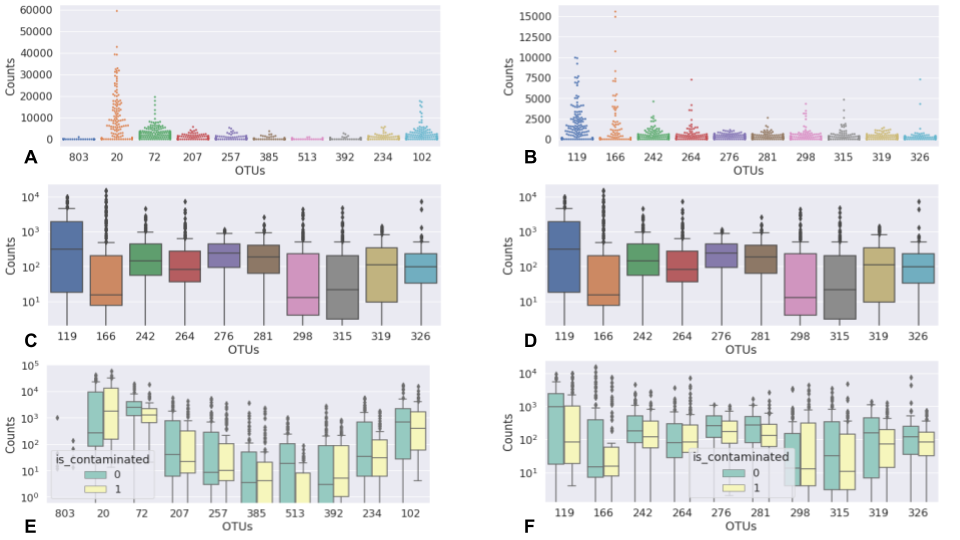
\includegraphics[ scale = 0.4]{./figs/plotsPraktikum.png}
		\caption{The beeswarmplot displays the AUCs for all prediction methods across all feature selection methods.}
	\end{figure}


\section{Diskussion}
%
Wichtiges Kennzeichen wissenschaftlichen Arbeitens ist die Trennung von Ergebnissen und deren Bewertung. Während im Abschnitt ``Ergebnisse'' entsprechend weitgehend auf Bewertungen verzichtet wird, findet die eigentliche Auswertung bzw. Interpretation der Ergebnisse in diesem Abschnitt statt. Ein weiteres Ziel ist eine kritische Reflexion der verwendeten Methodik. 

Bei der \textbf{Interpretation der Ergebnisse} sollten Sie regelmäßig Bezug auf die im Abschnitt ``Ergebnisse'' aufgeführten Tabellen oder Abbildungen nehmen. Eine bloße Zusammenfassung der erzielten Ergebnisse ist allerdings nicht ausreichend. Entscheidend ist vielmehr, die Ergebnisse einzuordnen und hinsichtlich ihrer Plausibilität sowie möglicher Fehler zu hinterfragen.
    
Bei der \textbf{Reflexion der Methoden} stellen Sie dar, inwieweit die von Ihnen gewählte Methodik dazu geeignet ist, die gewählte Fragestellung zu beantworten. Ein wichtiges wissenschaftliches Instrument dafür ist der Vergleich Ihrer Methode(n) mit einer oder mehreren Referenzmethoden. Es sollen sowohl Stärken bzw. Nutzen der Arbeit als auch deren Schwächen bzw. Grenzen dargestellt werden.
%
%
\section{Schlussfolgerungen}
%
Der letzte Abschnitt rundet die Arbeit mit einer zusammenfassenden Einordnung der erzielten Ergebnisse und der gewonnenen Erkenntnisse ab. Darin sollte insbesondere die im ersten Abschnitt eingeführte Forschungsfrage aufgegriffen und beantwortet werden. Im Idealfall wird darüber hinaus ein (kurzer) Ausblick auf potenzielle oder tatsächlich geplante weiterführende Arbeiten oder neue Fragestellungen gegeben, die sich aus der vorliegenden Arbeit ergeben.


%
% ---- Bibliography ----
%
%
\bibliographystyle{plain}
\bibliography{Paperrunde.bib}


\end{document}
